\chapter{Modelação da Base de Dados}

\paragraph{}

Resumidamente a base de dados está representada da seguinte forma:

\begin{list}{\textbf{-}}{\textbf{TABELAS}}
\item \textbf{curso} - Representa os cursos leccionados
\item \textbf{ano\_lectivo} - Representa um ano lectivo
\item \textbf{utilizador} - todos os utilizadores ficam registados nesta tabela
\item \textbf{curso\_ano} - Representa um curso leccionado num determinado ano, nesta tabela fica representado o coordenador do curso nesse ano associando o id do respectivo user na tabela utilizador
\item \textbf{semestre} - Representa um semestre de um determinado ano lectivo
\item \textbf{disciplina} - Representa uma disciplina
\item \textbf{disciplina\_semestre} - Faz referencia a uma disciplina leccionada num determinado semestre
\item \textbf{Docente} - Representa um ou mais utilizadores designados como docentes de uma determinada disciplina
\item \textbf{aluno} - Representa uma matrícula de um utilizador como aluno num determinado curso
\item \textbf{matricula\_disciplina} - Representa a matricula numa disciplina de um determinado aluno
\item \textbf{avaliacao} - Representa uma avaliacao marcada para uma disciplina leccionada num determinado semestre
\item \textbf{avaliacao\_datas\_alt} - Nesta tabela ficam registadas as datas alternati vas escolhidas pelo docente para que o coordenador possa ter a possibilidade de trocar caso aconteça um peso demasiado excessivo nas avaliações para os alunos.
\item \textbf{avaliacao\_aluno} - Representa a inscrição de um aluno numa avaliação e é onde fica registada a sua nota
\end{list}

\begin{list}{\textbf{-}}{\textbf{STORED PROCEDURES}}
\item \textbf{get\_coordinator\_evaluations( user\_num, num\_discipline )} - Obter lista de avaliações com o perfil de coordenador de um determinado utilizador
\begin{lstlisting}
DROP PROCEDURE IF EXISTS `get_coordinator_evaluations`$$
CREATE DEFINER=`moreira_aval`@`localhost` PROCEDURE `get_coordinator_evaluations`(IN user_num INT, num_discipline INT)
begin
SELECT 
	av.num_avaliacao as id, av.tipo_avaliacao as type, 
	av.peso as weight, av.data_avaliacao as date, av.activada as validated
	FROM avaliacao as av
	
	RIGHT JOIN (
		SELECT a.num_avaliacao	
		FROM curso_ano as ca
		LEFT JOIN disciplina d
			ON d.num_curso = ca.num_curso
		RIGHT JOIN avaliacao a
			ON a.num_disciplina = d.num_disciplina
		WHERE ca.num_coordenador = user_num
	) AS x 
	ON  x.num_avaliacao = av.num_avaliacao

	WHERE av.num_disciplina = num_discipline;
end$$
\end{lstlisting}

\item \textbf{get\_teacher\_evaluations( user\_num, num\_discipline )} - Obter lista de avaliações com o perfil de docente de um determinado utilizador
\begin{lstlisting}
DROP PROCEDURE IF EXISTS `get_teacher_evaluations`$$
CREATE DEFINER=`moreira_aval`@`localhost` PROCEDURE `get_teacher_evaluations`(IN user_num INT, num_discipline INT)
begin
SELECT 
	av.num_avaliacao as id, av.tipo_avaliacao as type, 
	av.peso as weight, av.data_avaliacao as date, av.activada as validated
	FROM avaliacao as av
	RIGHT JOIN (
		SELECT a.num_avaliacao
		FROM docente d
		LEFT JOIN avaliacao a
			ON a.num_disciplina = d.num_disciplina
			AND a.num_semestre = d.num_semestre
		WHERE d.num_utilizador = user_num
		AND a.num_disciplina = num_discipline
	) AS x 
	ON  x.num_avaliacao = av.num_avaliacao
	WHERE av.num_disciplina = num_discipline;
end$$
\end{lstlisting}

\item \textbf{get\_student\_evaluations( user\_num, num\_discipline )} - Obter lista de avaliações com o perfil de aluno de um determinado utilizador
\begin{lstlisting}
DROP PROCEDURE IF EXISTS `get_student_evaluations`$$
CREATE DEFINER=`moreira_aval`@`localhost` PROCEDURE `get_student_evaluations`(IN user_num INT, num_discipline INT)
begin
SELECT 
	av.num_avaliacao as id, av.tipo_avaliacao as type, 
	av.peso as weight, av.data_avaliacao as date, x.validated
	FROM avaliacao as av
	LEFT JOIN (
		SELECT a.num_avaliacao, 1 as validated	
		FROM avaliacao_aluno a
		WHERE a.num_utilizador = user_num
		AND a.num_disciplina = num_discipline
	) AS x 
	ON  x.num_avaliacao = av.num_avaliacao
	WHERE av.num_disciplina = num_discipline
	AND av.activada = 1;
end$$
\end{lstlisting}

\item \textbf{get\_cursos\_user( user\_num )} - Obter lista de cursos a que utilizador esteja associado
\begin{lstlisting}
DROP PROCEDURE IF EXISTS `get_cursos_user`$$
CREATE DEFINER=`moreira_aval`@`localhost` PROCEDURE `get_cursos_user`(IN user_num INT)
begin
SELECT c.num_curso as id, c.nome_curso as name, a.titulo_ano as year, x.role
	FROM curso_ano as ca
	RIGHT JOIN (
		SELECT a.num_curso, 'student' as role				FROM aluno a
		WHERE a.num_utilizador = user_num
		UNION (
			SELECT d.num_curso, 'teacher' as role
			FROM docente dc
				LEFT JOIN disciplina d
				ON d.num_disciplina = dc.num_disciplina
				WHERE dc.num_utilizador = user_num
		)
		UNION (
			SELECT c.num_curso, 'coordinator' as role
			FROM curso_ano as c
			WHERE c.num_coordenador = user_num
		)
			) as x
		ON x.num_curso = ca.num_curso
			LEFT JOIN ano_lectivo a
			on a.num_ano = ca.num_ano
LEFT JOIN curso c
ON c.num_curso = ca.num_curso;
end$$
\end{lstlisting}

\item \textbf{get\_coordinator\_disciplines( user\_num, num\_course )} - Obter lista de disciplinas com o perfil de coordenador de um determinado utilizador
\begin{lstlisting}
DROP PROCEDURE IF EXISTS `get_coordinator_disciplines`$$
CREATE DEFINER=`moreira_aval`@`localhost` PROCEDURE `get_coordinator_disciplines`(IN user_num INT, num_course INT)
begin
SELECT d.num_disciplina as id, d.descricao as description, d.titulo as title
	FROM disciplina d
	RIGHT JOIN curso_ano ca
	ON ca.num_curso = d.num_curso
	AND ca.num_coordenador = user_num
	WHERE d.num_curso = num_course;
end$$
\end{lstlisting}

\item \textbf{get\_teacher\_disciplines( user\_num, num\_course )} - Obter lista de disciplinas com o perfil de docente de um determinado utilizador
\begin{lstlisting}
DROP PROCEDURE IF EXISTS `get_teacher_disciplines`$$
CREATE DEFINER=`moreira_aval`@`localhost` PROCEDURE `get_teacher_disciplines`(IN user_num INT, num_course INT)
begin
SELECT d.num_disciplina as id, d.descricao as description, d.titulo as title
	FROM disciplina d
	RIGHT JOIN docente dc
	ON dc.num_disciplina = d.num_disciplina
	AND dc.num_utilizador = user_num
	WHERE d.num_curso = num_course;
end$$
\end{lstlisting}

\item \textbf{get\_student\_disciplines( user\_num, num\_course )} - Obter lista de disciplinas com o perfil de aluno de um determinado utilizador
\begin{lstlisting}
DROP PROCEDURE IF EXISTS `get_student_disciplines`$$
CREATE DEFINER=`moreira_aval`@`localhost` PROCEDURE `get_student_disciplines`(IN user_num INT, num_course INT)
begin
SELECT d.num_disciplina as id, d.descricao as description, d.titulo as title
	FROM disciplina d
	RIGHT JOIN matricula_disciplina md
	ON md.num_disciplina = d.num_disciplina
	AND md.num_utilizador = user_num
	WHERE d.num_curso = num_course;
end$$
\end{lstlisting}

\item \textbf{add\_evaluation( user\_num, discipline\_id, date, weight, classroom, type, observations )} - Adicionar uma avaliação a uma determinada disciplina
\begin{lstlisting}
DROP PROCEDURE IF EXISTS `add_evaluation`$$
CREATE DEFINER=`moreira_aval`@`localhost` PROCEDURE `add_evaluation`(IN user_num INT(11), discipline_id INT(11), date DATE, weight INT(11), classroom VARCHAR(20), type VARCHAR(100), observations VARCHAR(1000))
begin
if (SELECT 1 FROM docente 
	where num_utilizador = user_num 
	AND num_disciplina = discipline_id) = 1 THEN 
begin
INSERT INTO avaliacao (num_disciplina, num_semestre, data_avaliacao, peso, sala, tipo_avaliacao, observacoes, activada) values (discipline_id, 1, date, weight, classroom, type, observations, 0); 
end;
end if;
end$$
\end{lstlisting}

\end{list}

\begin{figure}[!htbp]
\centering
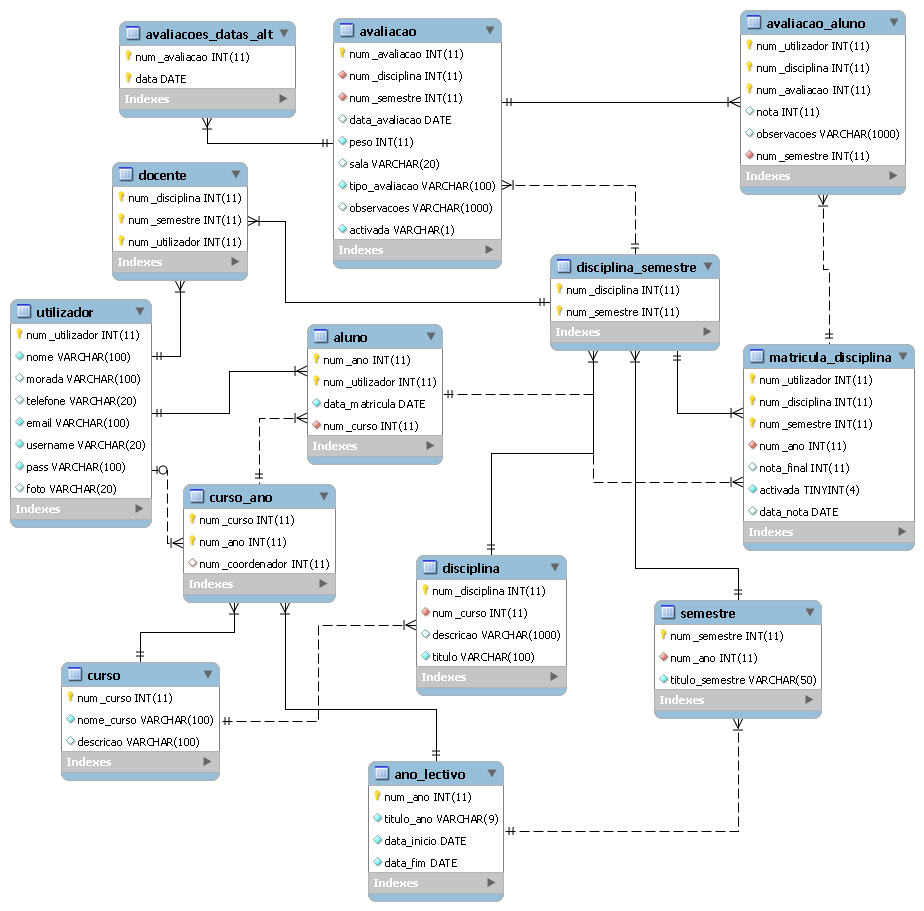
\includegraphics[width=17cm]{imagens/base_de_dados.png}
\caption{Base de Dados: Modelo Físico}
\label{fig:modelo_fisico}
\end{figure}

